\documentclass{beamer}

\usetheme{Warsaw}
\usecolortheme{seahorse}
\setbeamertemplate{navigation symbols}{}
\setbeamertemplate{caption}{\raggedright\scriptsize\insertcaption\par}
\setbeamertemplate{headline}{%
\leavevmode%
    \begin{beamercolorbox}[wd=\paperwidth,ht=3ex,dp=1.9ex]{palette quaternary}%
    \insertsectionnavigationhorizontal{\paperwidth}{\hskip0pt plus1fill}{\hskip0pt plus1fill}
    \end{beamercolorbox}%
}
\setbeamercolor{background canvas}{bg=}
\setlength{\parskip}{\medskipamount} 

% \setbeamerfont{footnote}{size=\tiny}
\usepackage{beamerthemesplit}
\usepackage{multicol}
\usepackage{lmodern}
\usepackage{bold-extra}
\usepackage{ragged2e}
\usepackage{pgf}
\usepackage[normalem]{ulem}
\usepackage{epsfig}
\usepackage{epstopdf}
\usepackage{graphicx}
\usepackage{tikz}
\usetikzlibrary{tikzmark}
\usepackage{slashbox}
\usepackage{amssymb}
\usepackage{xurl}
\usepackage{xcolor}
\usepackage{listings}
\usepackage{polski}
\usepackage[utf8]{inputenc}
\usepackage[absolute,overlay]{textpos}
\usepackage{minted}
\usepackage[style=numeric,backend=biber,sorting=none]{biblatex}
\usepackage[font=scriptsize,labelformat=empty,justification=centering]{caption}
\addbibresource{sdm2-2.bib}

% \let\olditem=\item
% \renewcommand{\item}{\olditem \justifying}
%
% \apptocmd{\frame}{}{\justifying}{}

\newcommand{\C}{\emph{C}}
\newcommand{\Esp}{\emph{ESP32}}
\newcommand{\Rpi}{\emph{RaspberryPi}}
\newcommand{\Cpp}{\emph{C++}}
\newcommand{\CLogo}{\raisebox{-0.25\totalheight}{\includegraphics[height=1.8\fontcharht\font`\B]{img/c-logo.png}}}
\newcommand{\Rust}{\emph{Rust}}
\newcommand{\Cargo}{\emph{Cargo}}
\newcommand{\RustLogo}{\raisebox{-0.25\totalheight}{\includegraphics[height=1.8\fontcharht\font`\B]{img/rust-logo.png}}}
\newcommand{\Zig}{\emph{Zig}}
\newcommand{\ZigLogo}{\raisebox{-0.25\totalheight}{\includegraphics[height=1.8\fontcharht\font`\B]{img/zig-logo.png}}}

\newcommand{\Modbus}{\emph{Modbus}}
% \newcommand{\Modbus}{\emph{MODBUS\textsuperscript{\copyright}}}
\newcommand{\Lizard}{\lstinline{lizard}}

\newcommand{\IR}{\bbold R}
\def\Rset{\mathbb{R}}
\def\Zset{\mathbb{Z}}
\newcommand{\refbr}[1]{(\ref{#1})}
\newcommand{\beq}{\begin{equation}}
\newcommand{\eeq}{\end{equation}}
\newcommand{\und}[1]{\underline{#1}}
\newcommand\pro{\item[$+$]}
\newcommand\con{\item[$-$]}
\newcounter{saveenumi}
\newcommand{\seti}{\setcounter{saveenumi}{\value{enumi}}}
\newcommand{\conti}{\setcounter{enumi}{\value{saveenumi}}}
\lstset{
    numbers=left,
    breaklines=true,
    tabsize=2,
	numberstyle=\color{gray}\footnotesize,
    basicstyle=\small\ttfamily,
}
\setminted{
    breaklines=true,
    tabsize=2,
    % bgcolor=lightgray,
    frame=single,
}

\newcommand{\ttbf}[1]{{\tt \textbf{#1}}}
\newcommand{\BeamerEnum}[1]{\usebeamertemplate{enumerate item}{\alph{#1}}}
% \AtBeginSection{
%   \begin{frame}
%   \vfill
%   \centering
%   \begin{beamercolorbox}[sep=8pt,center,shadow=true,rounded=true]{title}
%     \usebeamerfont{title}\insertsectionhead\par%
%   \end{beamercolorbox}
%   \vfill
%   \end{frame}
% }

\hypersetup{
   pdftitle={Analiza wybranych języków programowania na systemy wbudowane pod kątem wydajności i niezawodności},
   pdfauthor={Jakub Ostrzołek},
   pdfborder={0 0 0}
}

\title[Analiza języków dla systemów wbudowanych \insertframenumber/\inserttotalframenumber]{
	 Analiza wybranych języków programowania na systemy wbudowane pod
	 kątem wydajności i niezawodności
}
\author[Jakub Ostrzołek]{
 	\textbf{Jakub Ostrzołek} \\ \vspace{\smallskipamount}
	\scriptsize Kierunek: Informatyka, Inteligentne Systemy \\ \vspace{\bigskipamount}
  \footnotesize Promotor: dr inż. Patryk Chaber
}

\institute{
	Instytut Automatyki i Informatyki Stosowanej \\%
  Politechnika Warszawska
}

\begin{document}

\frame{\titlepage}

\frame{\tableofcontents\frametitle{Plan prezentacji}}

\section{Motywacja}

\begin{frame}
	\frametitle{Motywacja}

	\begin{columns}
		\column{\dimexpr\paperwidth-10pt}
		\begin{figure}
			\includegraphics[width=\linewidth]{img/plots/so-survey.pdf}
			\centering
			\caption{\citetitle{so-survey} \cite{so-survey}}
		\end{figure}
	\end{columns}
\end{frame}

\begin{frame}
	\frametitle{Trudności w \CLogo{} 1/2}

	\begin{columns}
		\column{\dimexpr\paperwidth-10pt}
		\begin{figure}
			\includegraphics[width=\linewidth]{img/plots/top-tags-c.pdf}
			\caption{Najpopularniejsze tagi zapytań z serwisu StackOverflow dla języka \C{} \cite{so-db}}
			\centering
		\end{figure}
	\end{columns}

\end{frame}

\begin{frame}
	\frametitle{Trudności w \CLogo{} 2/2}

	\begin{itemize}
		\item Zarządzanie pamięcią:
		      \begin{itemize}
			      \item Użycie po zwolnieniu (\emph{use after free}, \emph{double free}) % top 8 CWE
			      \item Przepełnienie bufora (\emph{buffer overflow}) % top 2,6 CWE
			      \item Jednoczesny dostęp
		      \end{itemize}
		\item Wartość zerowa (\emph{null safety}) % top 21 CWE
		\item Makra
		\item System budowania, menedżer pakietów
		\item Obsługa błędów
		\item Brak struktur/funkcji generycznych
	\end{itemize}
\end{frame}


\section{Wprowadzenie}

\begin{frame}
	\frametitle{Alternatywy}

	\begin{columns}[t]
		\begin{column}{.50\textwidth}
			\RustLogo{} \textbf{\Rust{}}
			\begin{itemize}
				\item Wydajność
				\item Bezpieczeństwo
				\item Produktywność
			\end{itemize}
			%
			% Oprócz tego
			% \begin{itemize}
			% 	\item Unikatowy \emph{,,Borrow checker''}
			% \end{itemize}
		\end{column}
		\begin{column}{.50\textwidth}
			\ZigLogo{} \textbf{\Zig{}}
			\begin{itemize}
				\item Prostota % przepływ kontroli, alokacje, brak makr
				      % \item Jawne alokacje
				\item Obliczenia w czasie kompilacji
				\item Interakcja z \C{}/\Cpp{} (FFI)
			\end{itemize}
		\end{column}
	\end{columns}

	\begin{block}{Inne możliwości}
		\begin{multicols}{2}
			\begin{itemize}
				\item \emph{C++}
				\item \emph{Python}
				\item \emph{Java} (Micronaut)
				\item \emph{Go}
				\item \emph{Ada}
				\item \emph{Lua}
			\end{itemize}
		\end{multicols}
	\end{block}
\end{frame}

\begin{frame}[containsverbatim]
	\frametitle{\RustLogo{} Rust 1/2}

	\begin{columns}
		\begin{column}{.50\textwidth}
			\begin{itemize}
				\item[\checkmark{}] Zarządzanie pamięcią $\rightarrow$ \emph{,,Borrow checker''}
				\item[\checkmark{}] \Cargo{} -- nowoczesny system budowania
				\item[\checkmark{}] Bezpieczniejsze makra
				      % \item[\checkmark{}] Wartość zerowa, obsługa błędów, struktury generyczne
			\end{itemize}

			\vspace{\bigskipamount}

			Wady
			\begin{itemize}
				\item[$-$] Wysoki poziom wejścia
			\end{itemize}
		\end{column}

		\begin{column}{.40\textwidth}
			\begin{minted}{rust}
let mut a = 1;

let r1 = &a;
let r2 = &a;
let r3 = &mut a;
			\end{minted}
			% println!(
			% 	"{}, {}, and {}",
			% 	r1, r2, r3
			% );

			\vspace{\bigskipamount}

			\begin{minted}[frame=leftline,rulecolor=red,framesep=\medskipamount,framerule=1pt,breakindent=0pt,breaksymbolleft=\phantom{},breaksymbolindentleft=0pt,breaksymbolindentright=0pt]{yaml}
cannot borrow `a` as mutable because it is also borrowed as immutable
		\end{minted}
		\end{column}
	\end{columns}

	\vspace{\bigskipamount}

\end{frame}

\begin{frame}
	\frametitle{\RustLogo{} Rust 2/2}

	\begin{columns}
		\column{\dimexpr\paperwidth-10pt}
		\begin{figure}
			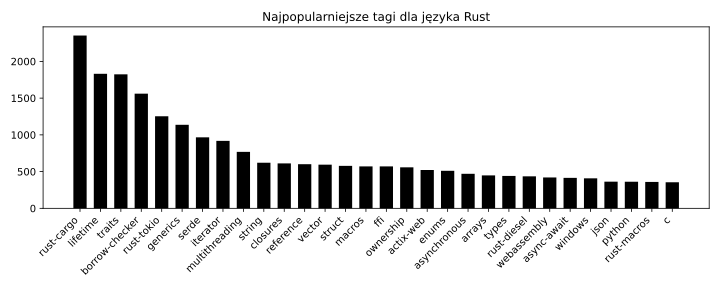
\includegraphics[width=\linewidth]{img/plots/top-tags-rust.pdf}
			\caption{Najpopularniejsze tagi zapytań z serwisu StackOverflow dla języka \Rust{} \cite{so-db}}
			\centering
		\end{figure}
	\end{columns}
\end{frame}

\begin{frame}[containsverbatim]
	\frametitle{\ZigLogo{} Zig 1/2}

	\begin{columns}
		\begin{column}{.50\textwidth}
			\begin{itemize}
				% \item[\checkmark{}] Prosty i spójny
				\item[\checkmark{}] Usprawnienia w zarządzaniu pamięcią
				\item[\checkmark{}] Obliczenia w czasie kompilacji
				      \begin{itemize}
					      \item \sout{makra}
					      \item \sout{strukt. generyczne}
				      \end{itemize}
				\item[\checkmark{}] \mintinline{zig}{@cInclude("modbus.h")}
			\end{itemize}

			\vspace{\bigskipamount}

			Wady
			\begin{itemize}
				\item[$-$] Młody -- częste zmiany
				\item[$-$] Mniej gwarancji niż \RustLogo{}
			\end{itemize}
		\end{column}

		\begin{column}{.60\textwidth}
			\begin{minted}{zig}
fn List(comptime T: type) type
{
    return struct {
        items: []T,
        len: usize,
    };
}

var list = List(i32){
    .items = &buffer,
    .len = 0,
};
			\end{minted}
		\end{column}
	\end{columns}

\end{frame}

\begin{frame}
	\frametitle{\ZigLogo{} Zig 2/2}

	\begin{columns}
		\column{\dimexpr\paperwidth-10pt}
		\begin{figure}
			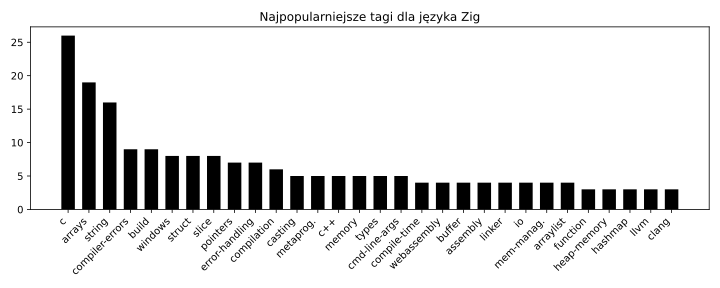
\includegraphics[width=\linewidth]{img/plots/top-tags-zig.pdf}
			\caption{Najpopularniejsze tagi zapytań z serwisu StackOverflow dla języka \Zig{} \cite{so-db}}
			\centering
		\end{figure}
	\end{columns}
\end{frame}

% \begin{frame}
% 	\frametitle{Porównanie zapytań (1/3)}
%
% 	\begin{figure}
% 		\includegraphics[width=0.8\linewidth]{img/plots/issues-0-totals.pdf}
% 		\caption{Łączna liczność zapytań z serwisu StackOverflow \cite{so-db}}
% 		\centering
% 	\end{figure}
% \end{frame}

\begin{frame}
	\frametitle{Porównanie zapytań (1/2)}

	\begin{figure}
		\includegraphics[width=\linewidth]{img/plots/issues-1.pdf}
		\caption{Liczność zapytań z serwisu StackOverflow dla wybranych tagów \cite{so-db}}
		\centering
	\end{figure}
\end{frame}

\begin{frame}
	\frametitle{Porównanie zapytań (2/2)}

	\begin{figure}
		\includegraphics[width=\linewidth]{img/plots/issues-2.pdf}
		\caption{Liczność zapytań z serwisu StackOverflow dla wybranych tagów \cite{so-db}}
		\centering
	\end{figure}
\end{frame}

\section{Cele pracy}

\begin{frame}
	\frametitle{Cel pracy}
	Porównanie ilościowe i jakościowe wybranych języków w praktycznych
	zastosowaniach dla systemów wbudowanych pod kątem:

	\begin{itemize}
		\item wydajności,
		\item bezpieczeństwa,
		\item produktywności.
	\end{itemize}
\end{frame}

\begin{frame}[containsverbatim]
	\frametitle{Metryki}

	\begin{columns}
		\begin{column}{0.5\linewidth}
			Statyczne:
			\begin{itemize}
				\item Rozmiar pliku binarnego
				\item Złożoność cyklometryczna (zmodyfikowana) (CNN')
				\item Liczba linii kodu bez komentarzy (NLOC)
				\item Liczba tokenów z leksera
			\end{itemize}

			Dynamiczne:
			\begin{itemize}
				\item Czas wykonania iteracji
				\item Zajętość stosu
				\item Zajętość sterty
			\end{itemize}
		\end{column}
		\begin{column}{0.5\linewidth}

			\vspace{\bigskipamount}

			\begin{minted}[escapeinside=??]{c}
void ?\tikzmark{func}?func(int a, int c) {
	?\tikzmark{whilee}?while (TRUE) {
		int b = get_b();
		?\tikzmark{iff}?if (a < b &&?\tikzmark{and}? c)
			break;
	}
}
			\end{minted}

			\begin{tikzpicture}[remember picture,overlay]
				\tikzset{every node/.style={inner sep=2pt}}
				\draw[red, <-] ([yshift=0.5em]pic cs:func) -- ++(135:.5)
				node[draw,red,fill=white,circle,font=\small,above left] {+1};
				\draw[red, <-] ([yshift=0.2em,xshift=-0.1em]pic cs:whilee) -- ++(180:.5)
				node[draw,red,fill=white,circle,font=\small,left] {+1};
				\draw[red, <-] ([yshift=0.2em,xshift=-0.1em]pic cs:iff) -- ++(180:.5)
				node[draw,red,fill=white,circle,font=\small,left] {+1};
				\draw[red, <-] (pic cs:and) -- ++(-45:.5)
				node[draw,red,fill=white,circle,font=\small,below right] {+1};
			\end{tikzpicture}

			\begin{align*}
				CNN(func)  & = 1+1+1+1 = 4 \\
				CNN'(func) & = 3
			\end{align*}

		\end{column}
	\end{columns}

\end{frame}

\begin{frame}
	\frametitle{Scenariusze testowe}
	\begin{enumerate}
		\item Kontrola diody LED (,,stroboskop''):
		      \begin{itemize}
			      \item ustawienie środowiska, interakcja z modułem GPIO.
		      \end{itemize}
		\item Kontrola silnika za pomocą potencjometru:
		      \begin{itemize}
			      \item interakcja z modułami: ADC oraz PWM.
		      \end{itemize}
		\item Regulacja PID obrotów silnika z komunikacją protokołem \Modbus{}:
		      \begin{itemize}
			      \item interakcja z modułami sieciowymi i biblioteką serwera \Modbus{},
			      \item precyzyjny podział czasu procesora,
			      \item realne obliczenia.
			            % \item dodatkowo potrzebny klient \Modbus{}.
		      \end{itemize}
	\end{enumerate}

	Realizacja na dwóch mikrokontrolerach:
	\begin{multicols}{2}
		\begin{itemize}
			\item \Rpi{} (+RPI OS),
			\item \Esp{} (+FreeRTOS).
		\end{itemize}
	\end{multicols}
\end{frame}

\begin{frame}
	\frametitle{Założenia}
	\begin{itemize}
		\item Identyczny układ sprzętowy dla każdego z języków
		\item Optymalizacje kompilacji dobrane pod metryki:
		      \begin{itemize}
			      \item Szybkość wykonania
			      \item Rozmiar pliku binarnego
		      \end{itemize}
		\item Pomiary uruchamiane wielokrotnie
		\item Czas na ,,rozgrzanie'' pamięci podręcznej
		\item Wykorzystanie analogicznych/identycznych rozwiązań (np. esp-idf, sys-fs)
	\end{itemize}
\end{frame}

\section{Wyniki}

\begin{frame}
	\frametitle{Scenariusz\BeamerEnum{\enumiii} -- regulator PID (schemat)}

	\begin{figure}
		\includegraphics[trim={0 1cm 0 0},clip,height=0.7\textheight]{../circuits/out/3-pid-bm-circuit.pdf}
		\caption{Schemat połączenia scenariusza\BeamerEnum{\enumiii} dla \Esp{}}
		\centering
	\end{figure}
\end{frame}

\begin{frame}
	\frametitle{Scenariusz\BeamerEnum{\enumiii} -- regulator PID (zachowanie)}

	Rdzeń 1 -- regulacja i interakcja ze sprzętem
	\begin{itemize}
		\item faza czytania (1 kHz): czujnik Halla
		\item faza regulacji (10 Hz):
		      \begin{itemize}
			      \item obliczanie sterowania
			      \item odczyt/zapis rejestrów \Modbus{}
		      \end{itemize}
	\end{itemize}
	Rdzeń 2 - interakcja ze światem
	\begin{itemize}
		\item stos sieciowy
		\item obsługa zapytań \Modbus{}
	\end{itemize}
\end{frame}

\begin{frame}[containsverbatim]
	\frametitle{Fragmenty kodu 1/2 -- \CLogo{}}
	\begin{minted}{c}
esp_err_t err = nvs_flash_init();
if (err != ESP_OK)
	return err;

err = esp_event_loop_create_default();
if (err != ESP_OK) {
	nvs_flash_deinit();
	return err;
}

err = my_mdns_init();
if (err != ESP_OK) {
	esp_event_loop_delete_default();
	nvs_flash_deinit();
	return err;
}
	\end{minted}
\end{frame}

\begin{frame}[containsverbatim]
	\frametitle{Fragmenty kodu 1/2 -- \ZigLogo{}}
	\begin{minted}{zig}
try idf.nvs_flash_init();
errdefer idf.nvs_flash_deinit();

try esp_event_loop_create_default();
errdefer sys.esp_event_loop_delete_default();

const mdns = try MDns.init();
errdefer mdns.deinit();
	\end{minted}
\end{frame}

\begin{frame}[containsverbatim]
	\frametitle{Fragmenty kodu 1/2 -- \RustLogo{}}
	\begin{minted}{rust}
let nvs = EspDefaultNvsPartition::take()?;

let sys_loop = EspSystemEventLoop::take()?;

let mdns = mdns_init()?;

// ... w bibliotece
impl<T: NvsPartitionId> Drop for EspNvs<T> {
	fn drop(&mut self) {
		unsafe { nvs_flash_deinit(self.1); }
	}
}
	\end{minted}
\end{frame}

\begin{frame}[containsverbatim]
	\frametitle{Fragmenty kodu 2/2 -- \CLogo{}}
	\begin{minted}{c}
esp_err_t read_phase(controller_t *self) {
	float value;
	esp_err_t err = read_adc(self, &value);
	if (err != ESP_OK)
		return err;

	if (value < treshold_close && !self->is_close) {
		self->is_close = true;
		*ringbuffer_back(self->revolutions) += 1;
	} else if (value > treshold_far && self->is_close){
		self->is_close = false;
	}

	return ESP_OK;
}
	\end{minted}
\end{frame}

\begin{frame}[containsverbatim]
	\frametitle{Fragmenty kodu 2/2 -- \ZigLogo{}}
	\begin{minted}{zig}
fn read_phase(self: *Self) !void {
	const value = try self.read_adc();

	if (value < treshold_close and !self.is_close) {
		self.is_close = true;
		self.revolutions.back().* += 1;
	} else if (value > treshold_far and self.is_close){
		self.is_close = false;
	}
}
	\end{minted}
\end{frame}

\begin{frame}[containsverbatim]
	\frametitle{Fragmenty kodu 2/2 -- \RustLogo{}}
	\begin{minted}{rust}
pub fn read_phase(&mut self) -> Result<()> {
	let value = self.read_adc()?;

	if value < treshold_close && !self.is_close {
		self.is_close = true;
		let back = self.revolutions.back_mut();
		*back += 1;
	} else if value > treshold_far && self.is_close {
		self.is_close = false;
	}

	Ok(())
}
	\end{minted}
\end{frame}

\begin{frame}
	\frametitle{Metryki statyczne}
	\begin{figure}
		\includegraphics[height=0.8\textheight]{img/plots/3-pid-bm.pdf}
		\centering
		\caption{Metryki statyczne scenariusza\BeamerEnum{\enumiii} dla \Esp{}}
	\end{figure}
\end{frame}

\begin{frame}
	\frametitle{Metryki dynamiczne}
	\begin{columns}
		\begin{column}{\dimexpr\paperwidth-10pt}
			\begin{figure}
				\includegraphics[width=\linewidth]{img/plots/3-pid-bm-perf.pdf}
				\centering
				\caption{Metryki dynamiczne scenariusza\BeamerEnum{\enumiii} dla \Esp{}}
			\end{figure}
		\end{column}
	\end{columns}
\end{frame}

\section{Wnioski}

\begin{frame}
	\frametitle{Wnioski}
	Nowoczesne języki programowania na systemy wbudowane:
	\begin{itemize}
		\item są bezpieczniejsze i wygodniejsze od \CLogo{}
		\item potrafią konkurować wydajnością z \CLogo{}
		\item dobrze współpracują z \CLogo{}
	\end{itemize}

	\vspace{\bigskipamount}

	Ale:
	\begin{itemize}
		\item rzadko mają bezpośrednie wsparcie twórców platformy
	\end{itemize}
\end{frame}

\begin{frame}
	\frametitle{Plan przyszłych prac}

	\begin{itemize}
		\item Zebranie metryk dynamicznych z wersji na \Rpi
		\item Analiza i sporządzenie dokumentu
	\end{itemize}
\end{frame}

\begin{frame}[allowframebreaks,noframenumbering]
	\frametitle{Bibliografia}
	\nocite{*}
	\printbibliography[heading=none]
\end{frame}

\end{document}
